\documentclass{beamer}

\usepackage[utf8]{inputenc}
\usepackage{default}

\title{All colours are beautiful}
\institute{MetaMeute}

\usetheme{Luebeck}

\begin{document}
\begin{frame}
 \maketitle
\end{frame}

\section{Bezugsquellendiskussion}
\begin{frame}
\begin{itemize}
 \item Angebote einholen
 \item Geldtransferkosten (Klassische Überweisung)
 \item Einfuhrumsatzsteuer
 \item Vor der Bestellung: Drei Wege Handshake
\end{itemize}
\end{frame}

\section{Aufbau}
\subsection{Strom}
\begin{frame}
\end{frame}

\subsection{Protokoll}
\begin{frame}
\begin{center}
 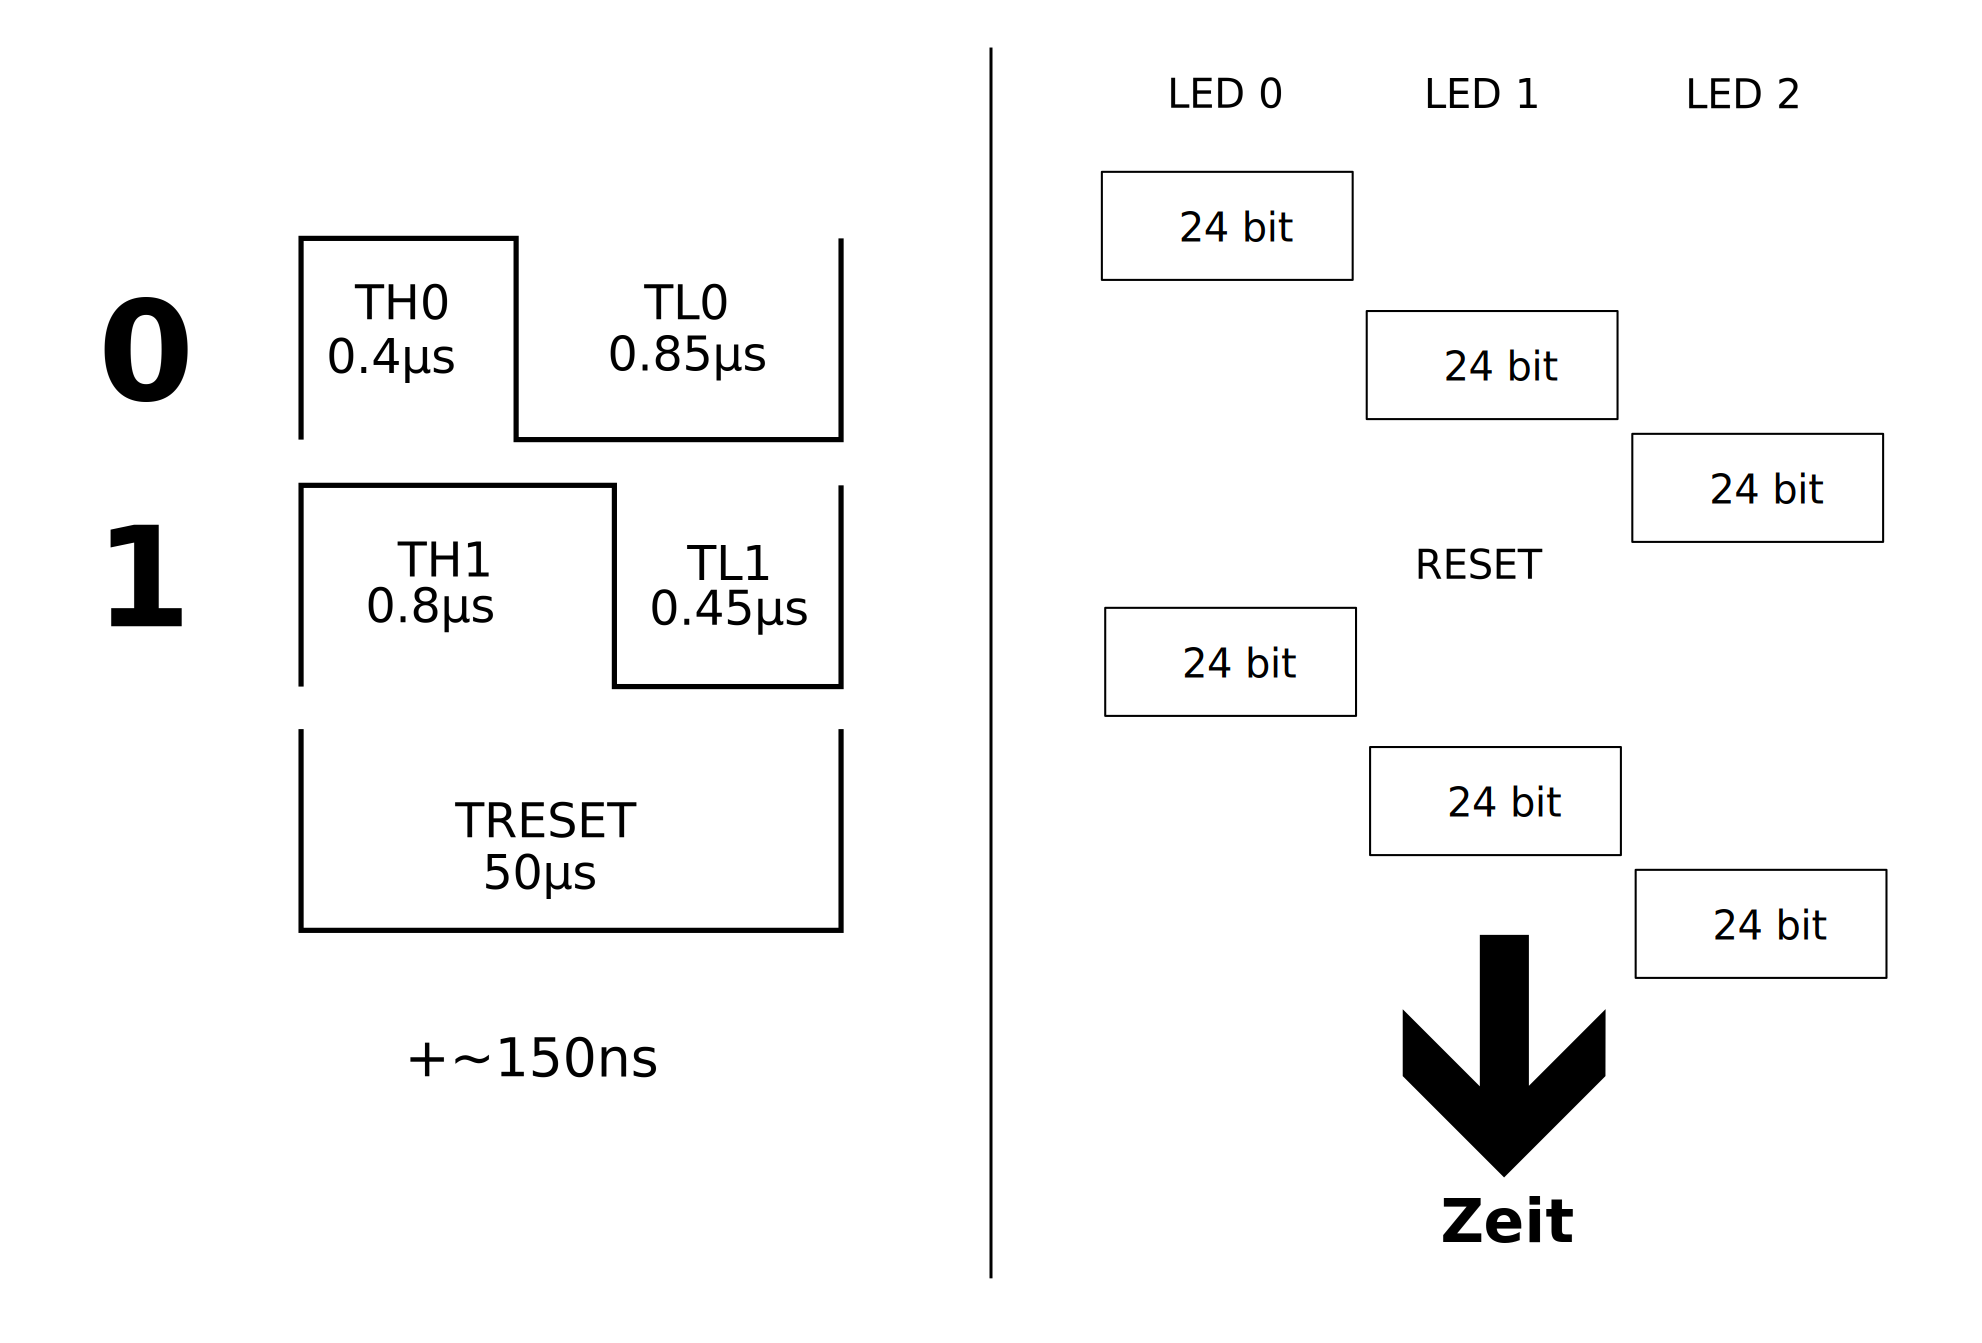
\includegraphics[width=11cm]{protokoll}
\end{center}
\end{frame}

\section{Ansteuerung}
\subsection{Arduino}
\begin{frame}
\end{frame}

\subsection{FTDI}
\begin{frame}{FTDI}
\end{frame}


\subsection{VoCore}
\begin{frame}{VoCore}
\end{frame}

\section{Projekte}
\subsection{Freifunk-Logo}
\begin{frame}
\end{frame}

\subsection{Musik-Visualisierung}
\begin{frame}
\end{frame}

\subsection{Lichtquelle}
\begin{frame}
\end{frame}

\section{Quellen}
\begin{frame}
 Hier Links zum git
\end{frame}


\end{document}
